\documentclass[20pt,margin=1in,innermargin=-4.5in,blockverticalspace=-0.25in]{tikzposter}
\geometry{paperwidth=42in,paperheight=30in}
\usepackage[utf8]{inputenc}
\usepackage{csquotes}
% \usepackage[estonian]{babel}
\usepackage{amsmath}
\usepackage{amsfonts}
\usepackage{amsthm}
\usepackage{amssymb}
\usepackage{mathrsfs}
\usepackage{graphicx}
\usepackage{adjustbox}
\usepackage{enumitem}
\usepackage{xcolor}
\usepackage[backend=biber,style=numeric]{biblatex}
\usepackage{unitartu-theme}
\usepackage{xeCJK}

\usepackage{mwe} % for placeholder images

\addbibresource{refs.bib}

% set theme parameters
\tikzposterlatexaffectionproofoff
\usetheme{UniTartuTheme}
\usecolorstyle{UniTartuStyle}

\usepackage[scaled]{helvet}
\renewcommand\familydefault{\sfdefault} 
\renewcommand{\vec}[1]{\bm{#1}}
\newcommand{\Tr}{\text{Tr}}
\usepackage[T1]{fontenc}


\title{B11 夫琅禾费圆孔衍射与菲涅尔圆孔衍射}
\author{\textbf{黄子维}\textsuperscript{1} 
% \quad \textbf{}\textsuperscript{2} % Add 2nd author
}
\institute{\textsuperscript{1}20980066,临床医学,中山大学中山医学院\\
            % \textsuperscript{2}Institute of Mathematics, University of Tartu % Add 2nd author institute
            }
\titlegraphic{\includegraphics[width=0.07\linewidth]{attachments//sysu.jpg}}

% begin document
\begin{document}
\maketitle
\centering
\begin{columns}
    \column{0.3}
    \block{实验背景}{
        光是一种横波,当光通过尺寸与其波长相近的圆孔时,将会发生圆孔衍射,形成明暗相间同心环状衍射条纹。根据入射光线是否为平行光,圆孔衍射又可分为夫琅禾费圆孔衍射(平行光圆孔衍射)和菲涅尔圆孔衍射(点光源衍射)。夫琅禾费圆孔衍射的中心条纹始终为亮纹,又称艾里斑,其半角范围为$\Delta \theta = 1.22 \frac{\lambda}{D}$。菲涅尔圆孔衍射中心条纹随圆孔直径或圆孔与观察屏距离改变而发生明暗变化,可由半波带数确定。\cite{cite:1}
        \vspace{2ex}
        
        为探究夫琅禾费圆孔衍射和菲涅尔圆孔衍射的图样和中心条纹的特征以及它们随实验参数改变而发生的变化,在本实验中,我们搭建光路,换用不同孔径的圆孔,观察夫琅禾费圆孔衍射和菲涅尔圆孔衍射图样,并使用光功率计测量了中心条纹的宽度。对于菲涅尔衍射,我们还改变了圆孔了观察屏的距离,以观察中心条纹的明暗变化。最后,我们在$Seelight$光学仿真平台上,使用同样的参数,进行了仿真实验。
    }
    \block{原理方法}{
        \vspace{-1em}
        \paragraph{\Large 实验光路装置图:}
        \vspace{1em}
        \begin{tikzfigure}[夫琅禾费圆孔衍射光路装置图]
        	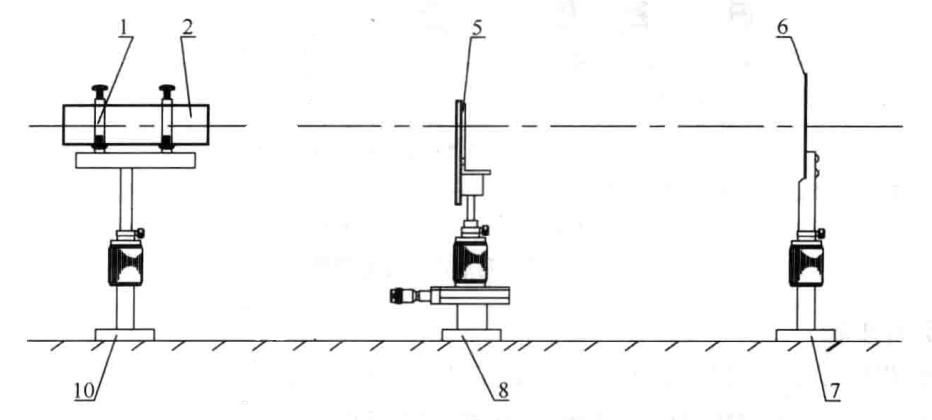
\includegraphics[width=0.6\linewidth]{attachments/illus-1.1.jpg}
        \end{tikzfigure}
        \vspace{1em}
        \begin{tikzfigure}[菲涅尔圆孔衍射光路装置图]
        	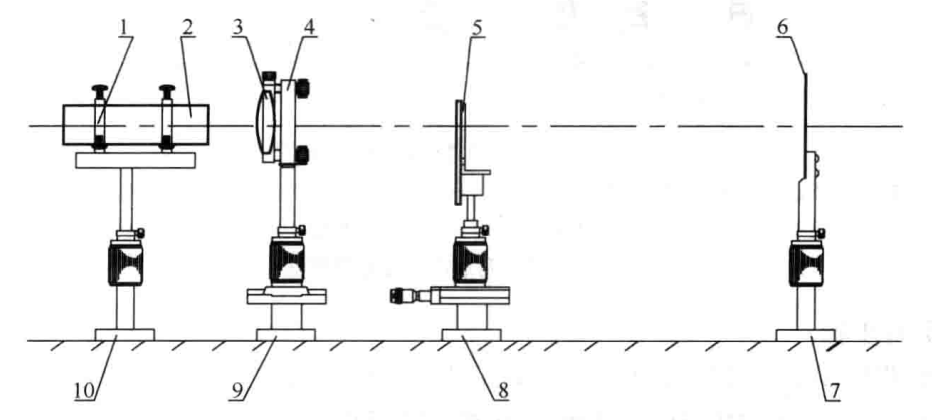
\includegraphics[width=0.6\linewidth]{attachments/illus-1.2.png}
        \end{tikzfigure}
        其中2,5,6分别为激光器,圆孔板和观察屏。3为扩束镜,仅在菲涅尔圆孔衍射中使用。
        \vspace{-1em}
        \paragraph{\Large 实验方法:}
            搭建光路,改变圆孔孔径,调节光路。在观察屏上获得衍射条纹后,换用光功率计,调节通用底座,在条纹中心附近找到光强极大值(或极小值),记录螺旋测微头读数。然后调节螺旋测微头,水平移动光功率计,直到第一次测量到光强极小值(或极大值),记录螺旋测微头读数。两示数之差即为中心条纹半径。
    }
    
    
%%%%%%%%%%%%%%%%%%% New Column
    \column{0.35}
    \block{夫琅禾费圆孔衍射实验结果}{
        观察不同孔径衍射图样,发现衍射图样中心条纹始终为亮纹。用光功率计测量中心亮斑半径,结果如表格所示。
        \vspace{1em}
        \begin{tikzfigure}[夫琅禾费圆孔衍射实验结果]
        	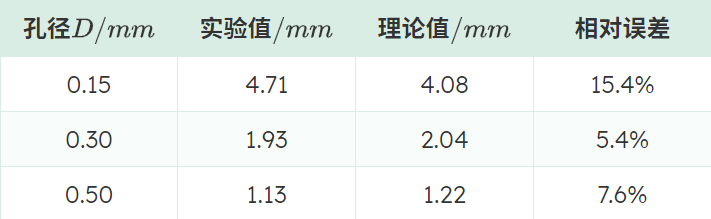
\includegraphics[width=0.6\linewidth]{attachments/tab-1.png}
        \end{tikzfigure}
        \vspace{1em}
        该实验中,0.15mm孔径测量误差较大,其余两组实验数据与理论值相符较好。推测因为0.15mm孔径下暗纹范围较宽,难以精确确定暗纹中心。
        \vspace{2ex}
        
        使用Seelight进行光学仿真,结果如下,与理论值符合较好
        \begin{tikzfigure}[夫琅禾费圆孔衍射仿真结果]
            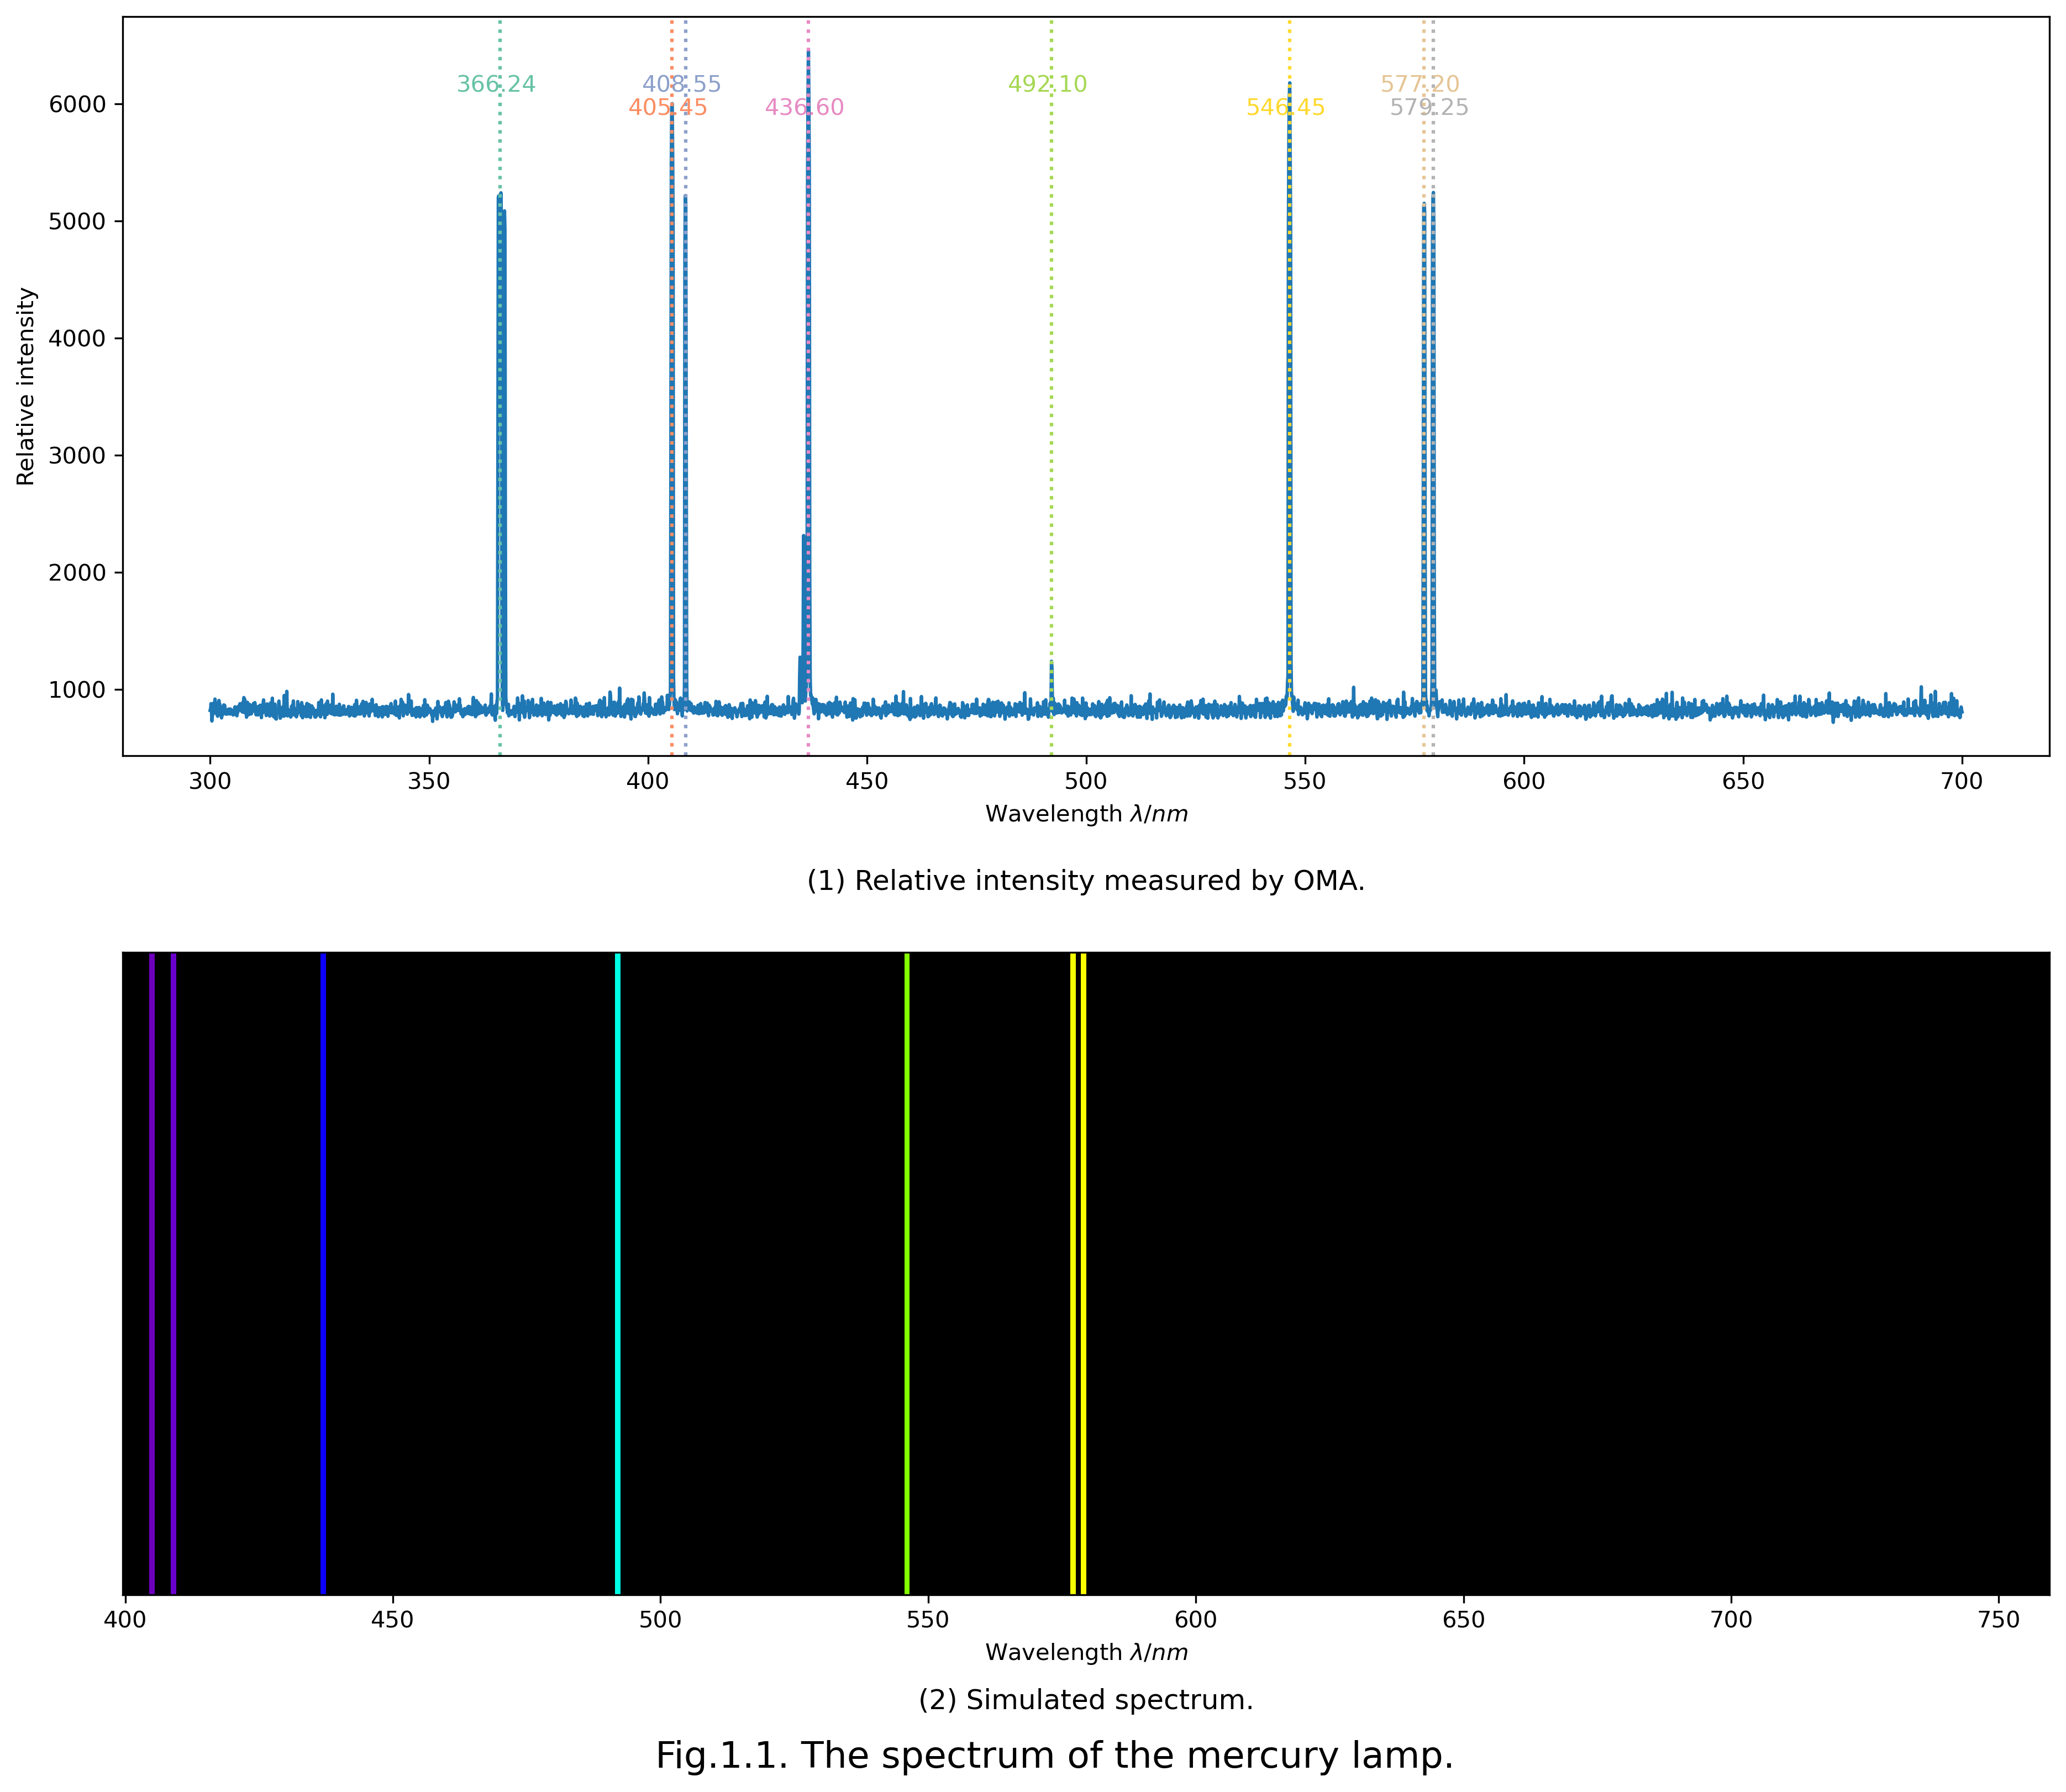
\includegraphics[width=0.9\linewidth]{attachments/Fig.1.1.png}
        \end{tikzfigure}
        \vspace{1em}
        
        仿真衍射图样如下,从左到右孔径分别为$0.15mm, 0.3mm, 0.5mm$
        \begin{tikzfigure}[夫琅禾费圆孔衍射仿真]
            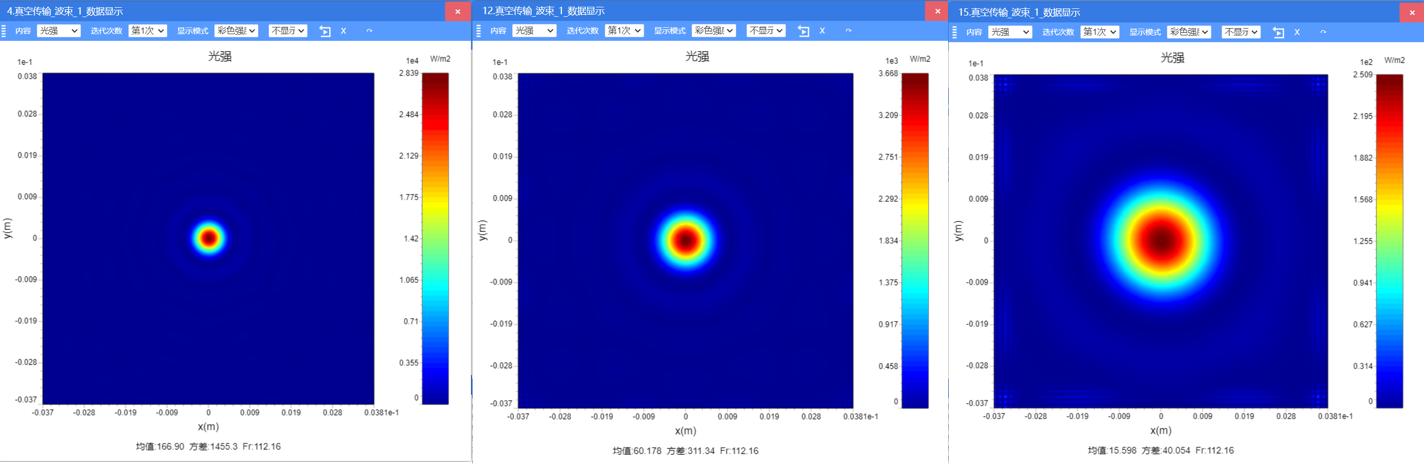
\includegraphics[width=0.9\linewidth]{attachments/Fig.1.2.png}
        \end{tikzfigure}
        \vspace{1em}
    }
    

    \column{0.35}
    \block{菲涅尔圆孔衍射实验结果}{
        观察不同孔径衍射图样,并改变圆孔到屏距离,发现衍射图样中心条纹随距离改变而发生亮暗变化。用光功率计测量中心亮斑半径,结果如表格所示。
        \vspace{1em}
        \begin{tikzfigure}[菲涅尔圆孔衍射实验结果]
        	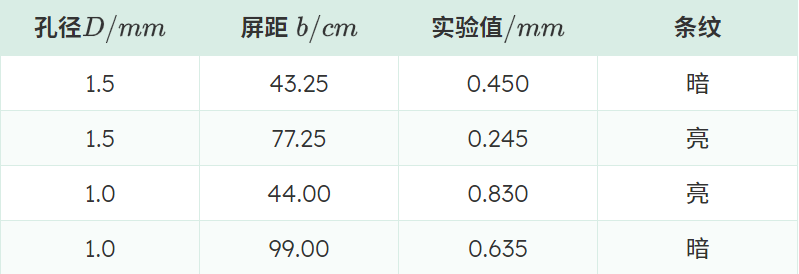
\includegraphics[width=0.55\linewidth]{attachments/tab-2.png}
        \end{tikzfigure}
        \vspace{1em}
        观察发现,在不同孔径下,改变屏孔距,中心条纹出现亮暗变化。对比两孔径,发现孔径越大,中心条纹半径越小。
        \vspace{2ex}
        
        使用Seelight进行光学仿真,结果如下
        \begin{tikzfigure}[菲涅尔圆孔衍射仿真]
            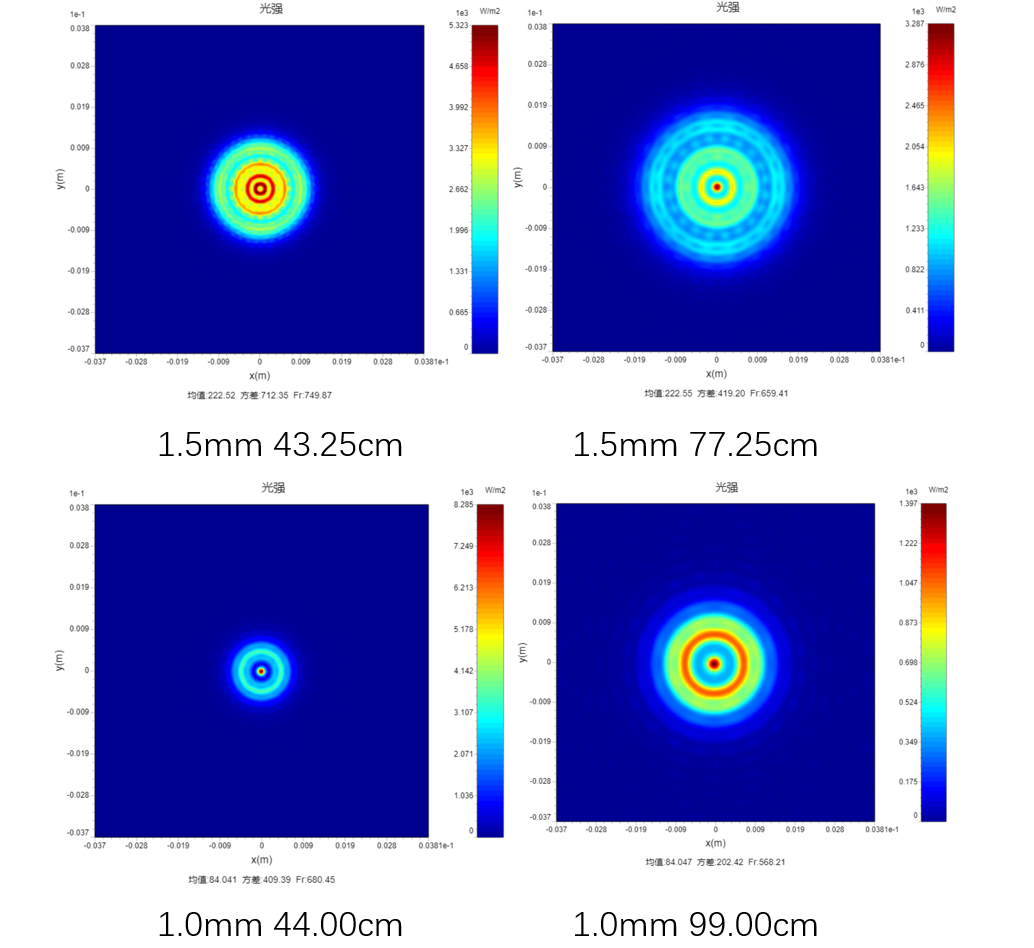
\includegraphics[width=0.5\linewidth]{attachments/Fig.2.2.png}
        \end{tikzfigure}
        \vspace{1em}
        
        仿真结果中,孔径$1.5mm$仿真结果中心亮暗纹情况与实验相符,但孔径$1.0mm$仿真结果中心均为亮纹,原因不明。
    }
    
    \block{实验结论}{
        本实验中,我们观察了夫琅禾费圆孔衍射和菲涅尔圆孔衍射,测量了中心条纹宽度并与实验值对比。通过实验,我们验证了夫琅禾费圆孔衍射中心始终为亮纹,而菲涅尔圆孔衍射中心条纹会随圆孔到观察屏距离改变而发生明暗变化。此外,我们的夫琅禾费圆孔衍射实验结果和理论值及仿真计算结果较好符合,但菲涅尔衍射实验与仿真结果并不完全符合,相关原因需要进一步研究。
    }
    
    \block{引用}{
        \vspace{-1em}
        \begin{footnotesize}
        \printbibliography[heading=none]
        \end{footnotesize}
    }
\end{columns}
\end{document}